% Options for packages loaded elsewhere
\PassOptionsToPackage{unicode}{hyperref}
\PassOptionsToPackage{hyphens}{url}
%
\documentclass[
]{book}
\usepackage{lmodern}
\usepackage{amssymb,amsmath}
\usepackage{ifxetex,ifluatex}
\ifnum 0\ifxetex 1\fi\ifluatex 1\fi=0 % if pdftex
  \usepackage[T1]{fontenc}
  \usepackage[utf8]{inputenc}
  \usepackage{textcomp} % provide euro and other symbols
\else % if luatex or xetex
  \usepackage{unicode-math}
  \defaultfontfeatures{Scale=MatchLowercase}
  \defaultfontfeatures[\rmfamily]{Ligatures=TeX,Scale=1}
\fi
% Use upquote if available, for straight quotes in verbatim environments
\IfFileExists{upquote.sty}{\usepackage{upquote}}{}
\IfFileExists{microtype.sty}{% use microtype if available
  \usepackage[]{microtype}
  \UseMicrotypeSet[protrusion]{basicmath} % disable protrusion for tt fonts
}{}
\makeatletter
\@ifundefined{KOMAClassName}{% if non-KOMA class
  \IfFileExists{parskip.sty}{%
    \usepackage{parskip}
  }{% else
    \setlength{\parindent}{0pt}
    \setlength{\parskip}{6pt plus 2pt minus 1pt}}
}{% if KOMA class
  \KOMAoptions{parskip=half}}
\makeatother
\usepackage{xcolor}
\IfFileExists{xurl.sty}{\usepackage{xurl}}{} % add URL line breaks if available
\IfFileExists{bookmark.sty}{\usepackage{bookmark}}{\usepackage{hyperref}}
\hypersetup{
  pdftitle={Migration Course},
  pdfauthor={Fränzi Korner \& Silke Bauer},
  hidelinks,
  pdfcreator={LaTeX via pandoc}}
\urlstyle{same} % disable monospaced font for URLs
\usepackage{color}
\usepackage{fancyvrb}
\newcommand{\VerbBar}{|}
\newcommand{\VERB}{\Verb[commandchars=\\\{\}]}
\DefineVerbatimEnvironment{Highlighting}{Verbatim}{commandchars=\\\{\}}
% Add ',fontsize=\small' for more characters per line
\usepackage{framed}
\definecolor{shadecolor}{RGB}{248,248,248}
\newenvironment{Shaded}{\begin{snugshade}}{\end{snugshade}}
\newcommand{\AlertTok}[1]{\textcolor[rgb]{0.94,0.16,0.16}{#1}}
\newcommand{\AnnotationTok}[1]{\textcolor[rgb]{0.56,0.35,0.01}{\textbf{\textit{#1}}}}
\newcommand{\AttributeTok}[1]{\textcolor[rgb]{0.77,0.63,0.00}{#1}}
\newcommand{\BaseNTok}[1]{\textcolor[rgb]{0.00,0.00,0.81}{#1}}
\newcommand{\BuiltInTok}[1]{#1}
\newcommand{\CharTok}[1]{\textcolor[rgb]{0.31,0.60,0.02}{#1}}
\newcommand{\CommentTok}[1]{\textcolor[rgb]{0.56,0.35,0.01}{\textit{#1}}}
\newcommand{\CommentVarTok}[1]{\textcolor[rgb]{0.56,0.35,0.01}{\textbf{\textit{#1}}}}
\newcommand{\ConstantTok}[1]{\textcolor[rgb]{0.00,0.00,0.00}{#1}}
\newcommand{\ControlFlowTok}[1]{\textcolor[rgb]{0.13,0.29,0.53}{\textbf{#1}}}
\newcommand{\DataTypeTok}[1]{\textcolor[rgb]{0.13,0.29,0.53}{#1}}
\newcommand{\DecValTok}[1]{\textcolor[rgb]{0.00,0.00,0.81}{#1}}
\newcommand{\DocumentationTok}[1]{\textcolor[rgb]{0.56,0.35,0.01}{\textbf{\textit{#1}}}}
\newcommand{\ErrorTok}[1]{\textcolor[rgb]{0.64,0.00,0.00}{\textbf{#1}}}
\newcommand{\ExtensionTok}[1]{#1}
\newcommand{\FloatTok}[1]{\textcolor[rgb]{0.00,0.00,0.81}{#1}}
\newcommand{\FunctionTok}[1]{\textcolor[rgb]{0.00,0.00,0.00}{#1}}
\newcommand{\ImportTok}[1]{#1}
\newcommand{\InformationTok}[1]{\textcolor[rgb]{0.56,0.35,0.01}{\textbf{\textit{#1}}}}
\newcommand{\KeywordTok}[1]{\textcolor[rgb]{0.13,0.29,0.53}{\textbf{#1}}}
\newcommand{\NormalTok}[1]{#1}
\newcommand{\OperatorTok}[1]{\textcolor[rgb]{0.81,0.36,0.00}{\textbf{#1}}}
\newcommand{\OtherTok}[1]{\textcolor[rgb]{0.56,0.35,0.01}{#1}}
\newcommand{\PreprocessorTok}[1]{\textcolor[rgb]{0.56,0.35,0.01}{\textit{#1}}}
\newcommand{\RegionMarkerTok}[1]{#1}
\newcommand{\SpecialCharTok}[1]{\textcolor[rgb]{0.00,0.00,0.00}{#1}}
\newcommand{\SpecialStringTok}[1]{\textcolor[rgb]{0.31,0.60,0.02}{#1}}
\newcommand{\StringTok}[1]{\textcolor[rgb]{0.31,0.60,0.02}{#1}}
\newcommand{\VariableTok}[1]{\textcolor[rgb]{0.00,0.00,0.00}{#1}}
\newcommand{\VerbatimStringTok}[1]{\textcolor[rgb]{0.31,0.60,0.02}{#1}}
\newcommand{\WarningTok}[1]{\textcolor[rgb]{0.56,0.35,0.01}{\textbf{\textit{#1}}}}
\usepackage{longtable,booktabs}
% Correct order of tables after \paragraph or \subparagraph
\usepackage{etoolbox}
\makeatletter
\patchcmd\longtable{\par}{\if@noskipsec\mbox{}\fi\par}{}{}
\makeatother
% Allow footnotes in longtable head/foot
\IfFileExists{footnotehyper.sty}{\usepackage{footnotehyper}}{\usepackage{footnote}}
\makesavenoteenv{longtable}
\usepackage{graphicx,grffile}
\makeatletter
\def\maxwidth{\ifdim\Gin@nat@width>\linewidth\linewidth\else\Gin@nat@width\fi}
\def\maxheight{\ifdim\Gin@nat@height>\textheight\textheight\else\Gin@nat@height\fi}
\makeatother
% Scale images if necessary, so that they will not overflow the page
% margins by default, and it is still possible to overwrite the defaults
% using explicit options in \includegraphics[width, height, ...]{}
\setkeys{Gin}{width=\maxwidth,height=\maxheight,keepaspectratio}
% Set default figure placement to htbp
\makeatletter
\def\fps@figure{htbp}
\makeatother
\setlength{\emergencystretch}{3em} % prevent overfull lines
\providecommand{\tightlist}{%
  \setlength{\itemsep}{0pt}\setlength{\parskip}{0pt}}
\setcounter{secnumdepth}{5}
\usepackage{booktabs}
\usepackage[]{natbib}
\bibliographystyle{apalike}

\title{Migration Course}
\author{Fränzi Korner \& Silke Bauer}
\date{2020-05-05}

\begin{document}
\maketitle

{
\setcounter{tocdepth}{1}
\tableofcontents
}
\hypertarget{prerequisites}{%
\chapter{Prerequisites}\label{prerequisites}}

This is a \emph{sample} book written in \textbf{Markdown}. You can use anything that Pandoc's Markdown supports, e.g., a math equation \(a^2 + b^2 = c^2\).

The \textbf{bookdown} package can be installed from CRAN or Github:

\begin{Shaded}
\begin{Highlighting}[]
\KeywordTok{install.packages}\NormalTok{(}\StringTok{"bookdown"}\NormalTok{)}
\CommentTok{# or the development version}
\CommentTok{# devtools::install_github("rstudio/bookdown")}
\end{Highlighting}
\end{Shaded}

Remember each Rmd file contains one and only one chapter, and a chapter is defined by the first-level heading \texttt{\#}.

To compile this example to PDF, you need XeLaTeX. You are recommended to install TinyTeX (which includes XeLaTeX): \url{https://yihui.name/tinytex/}.

\hypertarget{introduction}{%
\chapter{Introduction}\label{introduction}}

\hypertarget{course-schedule}{%
\section{Course schedule}\label{course-schedule}}

The course consists of lectures, student work on projects and visits to the ringing station. As the latter is dependent on weather, the following schedule is not entirely fixed but somewhat flexible.

Update for

\hypertarget{monday}{%
\subsection{Monday}\label{monday}}

\textbf{Morning} - Arrival

\textbf{Afternoon}

\hypertarget{tuesday}{%
\subsection{Tuesday}\label{tuesday}}

\hypertarget{wednesday}{%
\subsection{Wednesday}\label{wednesday}}

\hypertarget{thursday}{%
\subsection{Thursday}\label{thursday}}

\hypertarget{friday}{%
\subsection{Friday}\label{friday}}

\hypertarget{animal-migration}{%
\chapter{Animal migration}\label{animal-migration}}

\hypertarget{what-is-migration}{%
\section{What is migration?}\label{what-is-migration}}

Not all birds migrate and not all movements are migratory movements. The types of movements that exist range from:
1. local movements between roosting and feeding sites, movements within the home range
2. foraging journeys (e.g.~sea birds, swifts),\\
3. dispersal: juvenile (natal) dispersal, breeding dispersal,\\
4. migration, including its most common form of seasonal migration but also nomadism and irrup-tive migrations.

Migrations are persistent, directional movements from one destination to another, uninterrupted by intervening resources (Dingle 2014). The distances covered are often astounding, yet, the most ex-traordinary aspects of migration are perhaps the ubiquity of the phenomenon and the abundance of individuals involved. For instance, an estimated 1855 bird species (19\% of extant species) are migrato-ry. Of the avian species that use terrestrial and freshwater habitats, roughly 45\% of those breeding in North America undergo seasonal migration, and over 30\% breeding in the Palearctic migrate to sub-Saharan Africa, with many more migrating within Europe. Although accurate estimates of the number of individuals involved are scant, more than 2 billion passerine birds are found to migrate to sub-Saharan Africa, whereas upwards of 3 billion insects migrate over any 1-km stretch of countryside in southern England. Thus, Migration is set apart from the other movement types by i) its timing, frequency and predictability, ii) the intensity of interactions with resident species, and iii) the spatial scales over which they connect communities and ecosystems.

\hypertarget{why-do-birds-migrate}{%
\section{Why do birds migrate?}\label{why-do-birds-migrate}}

The classic bird migration is the biannual migration between breeding and non-breeding (`wintering') grounds. The breeding grounds are suitable for nesting and hatchling/fledgling survival, whereas the wintering grounds are more suitable for post-fledgling and adult survival. Migration is thought to be primarily an adaptation to the seasonality of resources - to use (a surplus of) resources that are only seasonally available and to avoid shortage of resources at specific times of the year.
Indeed, almost all places on Earth are seasonal to some degree and therefore, many migrants move between these seasonally available resources. For instance, many birds breeding in Europe migrate to the Sahel-zone in Africa in the Northern winter. The advantage of being in an area that provides better condition outweighs the cost of migration. In the temperate zones, it are usually those species that leave the breeding area during winter that have specific food requirements, which is not available dur-ing winter, e.g.~insects, but abundant in the Sahel after rainfall. Many species, e.g.~the Red-backed shrike Lanius collurio (Tøttrup et al.~2012), migrate within the non-breeding season between distinct non-breeding areas in order to make use of seasonally changing food availability.\\
There may be also other forms of migration or migrations as a strategy to avoid predator sor patho-gens.
Other migration than seasonal migration are moult and facultative migrations. In moult migrations, birds appear to migrate to predator-free areas where they can safely shed their flight feathers. In facultative migrations, birds only migrate long-distances when food is sparse, e.g.~many finches (Newton 2006). At an extreme end of the spectrum are birds that are nomadic, like grey teal (Anas gracilis) looking for ephemeral water and food sources in a desert landscape in Australia.
Two main flight modes exist -- flapping and soaring, which has consequences on when and where birds migrate: Flapping flight is energetically costly but can be used under a wide range of weather and topographic conditions, whereas for soaring thermals or wind are needed.
The majority of birds cannot feed while flying, and in many cases the total travel distance exceeds the maximum flight distance. Thus, the birds need stop-over sites in between, where they can replenish their reserves. A good example are tundra swans (Cygnus columbianus) that migrate between 4000-5500 km, whereas the maximally recorded non-stop flight is 2850 km. These swans mainly refuel on energy-rich, belowground parts of macrophytes in shallow lakes and wetlands along the route.

\begin{figure}

{\centering 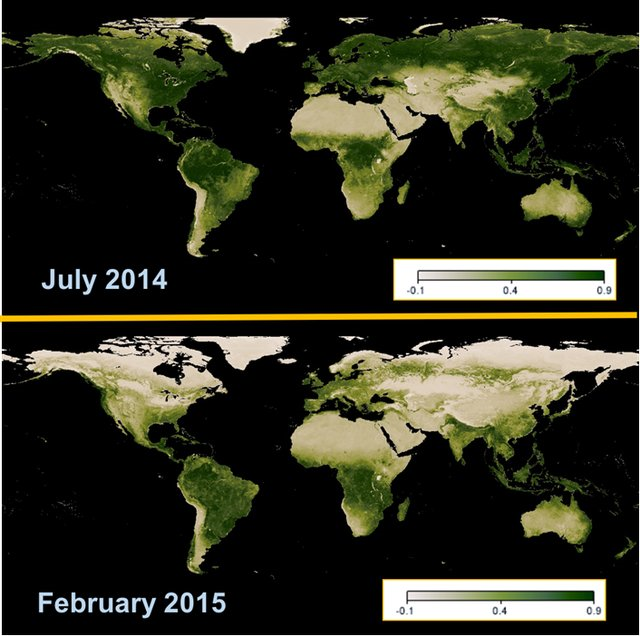
\includegraphics[width=1\linewidth]{figures/Fig_SeasonalChanges_NDVI} 

}

\caption{Seasonal change in global NDVI. These vegetation maps were generated from MODIS/Terra measurements of the Normalized Difference Vegetation Index (NDVI). Significant seasonal variations in the NDVI are apparent between northern hemisphere summer (July 2014; top) and winter (February 2015; bottom). Image credit: Reto Stockli, NASA Earth Observatory Group, using data from the MODIS Land Science Team (http://neo.sci.gsfc.nasa.gov).}\label{fig:unnamed-chunk-1}
\end{figure}

\hypertarget{terminology-of-specific-migration-patterns}{%
\section{Terminology of specific migration patterns}\label{terminology-of-specific-migration-patterns}}

There is a variety of migration patterns of which some are also tagged with specific terms. Often it is a specific characteristic or pattern that is emphasized, e.g.~the difference in distances covered led to the distinction of short- and long-distance migrants. However, the terminology is not very consistent and may be confusing at the beginning; we explain the most-often used terms below.

Box 1. Terminology for specific migration characteristics and patterns and a few examples.

\textbf{Short-distance migration} Migration over `shorter' distances, typically \textless5000kms, e.g.~from Central Europe to the Mediterranean. Sometimes, short-distance migrants are also partial migrants. Starling Sturnus vulgaris

\textbf{Long-distance migration} Migration over longer distances, usually \textgreater5000kms and often including the crossing of ecological barriers such as mountains, seas or deserts. Arctic tern Sterna paradisaea, Barn Swallow Hirundo rustica

\textbf{Nomadism} Irregular (not every year) movements to new breeding or non-breeding areas depending on food availability or other environmental conditions. Crossbill Loxia curvirostra

\textbf{Irruptive migration} Migration of unusually many individuals of one species. Of-ten from north to south in autumn after a good breeding sea-son and a cold spell; usually do not occur every year, but can be relatively regular and synchronized between species (Korner-Nievergelt et al.~2008). Great tit Parus major, Coal tit Parus ater

\textbf{Moult migration} Migration after the breeding season to distinct places where the birds moult before autumn migration. Goosanders Mergus merganser (European populations moult in northern Norway)

\textbf{Leap-frog migrations} Populations breeding further north spend the non-breeding season further south than breeding populations from further south. Thus, some populations ``overtake'' others on migra-tion. European robin Eritha-cus rubecula (Korner-Nievergelt et al.~2014)

\textbf{Chain migration} Northern breeding populations spend the non-breeding peri-od in breeding areas of southern populations. Thus, a spe-cies can be observed year-round but it are different individu-als in winter/ summer. Cormorant Phalacrocorax carbo (Fred-eriksen et al.~2018)

\textbf{Broad front migration} Individuals disperse over the whole distributional range while migrating (theoretically a lot of parallel flight tracks dispersed over a large area). Yet, migrants can still accumulate de-pending on topography and funnel through narrow areas. Chaffinch Fringilla coe-lebs, many passerines: (Liechti et al.~1996)

\textbf{Funnel migration} All individuals of a species (or population) concentrate on migration in one stop over area or a topographically im-portant place such as Gibraltar. Crane Grus grus, many waders (Yellow sea!)

\textbf{Nocturnal migration} Most songbirds migrate at night, i.e.~they are nocturnal mi-grants. This behavior has been attributed to reduced preda-tion risk, good flight conditions, or for saving the daylight for feeding. Nocturnal migrants mostly fly alone or in loose flocks. Most migratory song-birds, e.g.~Wheatear Oenanthe oenanthe

\textbf{Diurnal migration} Migratory flights take place during the day. Many larger birds are diurnal migrants, e.g.~birds of prey that use thermals or swans and geese that often fly in flocks. Red kites, bee-eaters, many geese species

\textbf{Partial migration} Only a part of a population migrates while the remaining part stays resident. Which individuals stay and which migrate has often a genetic background, and in some years, the migrato-ry part enjoys a fitness benefit while in other years the resi-dents are better off.

\hypertarget{importance-of-migration-for-the-structure-and-dynamics-of-resident-communities}{%
\section{Importance of migration for the structure and dynamics of resident communities}\label{importance-of-migration-for-the-structure-and-dynamics-of-resident-communities}}

The number of migrant populations often exceeds those of resident species. For instance, we estimat-ed the number of (passerine) birds migrating between Europe and Africa to be impressive 2.1. billion individuals (Hahn et al.~2009)! To cross the Sahara on their way to Africa, they need the energy of 34'000 tons of insects, 36'000 tons of fruit and 2'000 tons of seeds.
If we consider migrants more generally, i.e.~beyond birds, we find that migrants transport nutrients, energy, and other organisms (including seeds, mollusks, parasites, and pathogens) between disparate locations. Migrants also forage and are preyed upon throughout their journeys, thereby establishing transport and trophic interactions with resident communities. Migratory animals thus couple ecological communities across the globe and may mediate their diversity and stability. However, as yet, the influ-ence of migrants and their services on these communities is often overlooked, and as a consequence of global changes, migrations are threatened worldwide.

Through these transport and trophic effects, migrants interact with resident communities. For instance, they may uniquely alter energy flow, food-web topology and stability, trophic cascades, and the struc-ture and dynamics of (meta-)communities. For example, the inputs of nutrients and energy originating from distant localities by migrants can dramatically increase resource availability, with rippling conse-quences for productivity at various trophic levels and the potential to drive the transition between alter-native stable states. Migrant-mediated transport of propagules of other organisms can lead to the es-tablishment of new or lost species, as well as influencing gene fl ow and genetic mixing among resident populations. Similarly, migrants can alter parasite transmission, diversity, and evolution by harboring a broader range of parasites than residents and by either facilitating or hindering the longdistance dis-persal of parasites. Foraging by migrants can also have profound effects on community processes and ecosystem functions. For instance, grazing by migratory animals can alter nutrient cycling, primary productivity, biomass of edible plants, competitive interactions between plant species, and ultimately, the composition and long-term persistence of the entire plant community. The most striking difference between migrant and resident consumers is, however, the pulsed nature of migrant utilization and the timing of their interactions. Together, these fundamentally defi ne the relationship between migrant abundance and primary production (in the case of migrant herbivores) or the stability of food webs (in the case of migratory predators).

The highly predictable, seasonally pulsed nature of animal migration, together with the spatial scales at which it operates and the immense number of individuals involved, not only set migration apart from other types of movement, but render it a uniquely potent, yet underappreciated, dimension of biodiver-sity that is intimately embedded within resident communities. Given the potential for migration to influ-ence ecological networks worldwide, we suggest integrative network approaches, through which stud-ies of community dynamics and ecosystem functioning may explicitly consider animal migrations, un-derstand the ramifications of their declines, and assist in developing effective conservation measures.

\hypertarget{timing-of-migration}{%
\chapter{Timing of migration}\label{timing-of-migration}}

\hypertarget{why-is-timing-important}{%
\section{Why is timing important?}\label{why-is-timing-important}}

The timing of migration (and other life-history activities) is widely considered to have significant fitness consequences (Forrest \& Miller-Rushing 2010, Miller-Rushing \& et al.~2010). Particularly in seasonal environments, timing is the all-dominant predictor of success -- for instance migration, growth or repro-duction should coincide with favourable conditions and avoid unfavourable periods. Thus, such activi-ties need to be initiated within a specific -- often very restricted -- time frame.
Penalties for not migrating at the optimal time range from slight reductions in reproductive success (e.g.~raising fewer offspring or offspring with lower survival prospects) to fatal consequences (e.g.~mistiming of migration leading to starvation (Newton 2007). Besides immediate penalties there may also be time-lagged consequences (e.g.~carry-over effects; Harrison et al.~2011), since current mistiming may bear a cost later in life.

\hypertarget{what-determines-the-timing-of-migratory-steps-cues}{%
\section{What determines the timing of migratory steps? Cues!}\label{what-determines-the-timing-of-migratory-steps-cues}}

Photoperiod has been shown to be involved in the timing of activities for many species, e.g.~initiating ``Zugunruhe'' or determining the speed of migratory progression, as it indicates time of the year and thus, can be a useful predictor for the phenology of resources (Fig. 1). Other, local and short-term fac-tors influencing timing of migration include prevailing weather conditions, e.g.~temperature, wind, drought and precipitation, as these factors can significantly influence the costs of the travel ahead or its consequences for survival. There are also internal cues that serve as a clock or time-keeping mecha-nism. Additionally, physiological state and developmental stage are important cues as most migrants undergo morphological and physiological changes in preparation for migration and internal signals, e.g.~hormone levels, indicate when these changes are completed.
Migration can be divided into a few major steps -- preparation, departure, on the way, and ter-mination -- a cycle that might be repeated if migration is suspended at intermittent stop-over sites. Each of these steps potentially requires specific cues and decision rules as the demands on the animal's physiology and behaviour differ. Similarities might exist across taxonomic groups in how animals deal with each of these steps but differences may also be expected depending on the specific way of mi-grating or their particular environment.

\hypertarget{preparation}{%
\subsection{Preparation}\label{preparation}}

Before actually embarking on migration, most birds (partly) change the composition of their bodies, e.g.~increase flight muscles at the expense of leg muscles, atrophy digestive and metabol-ic organs (Piersma \& van Gils 2011) and accumulate body stores. Photoperiod is an important external signal for preparations; it initiates ``Zugunruhe'', i.e.~migratory restlessness (Gwinner 1990), and birds start accumulating body stores, altering their digestive system and building up flight muscles from a particular day length onwards. The specific value of day length, at which these transformations are started, is under strong genetic control (Newton 2008:324).
However, also birds kept under constant day length for up to several years still showed a cir-cannual rhythm with the right sequence of annual events (migratory fat deposition and restlessness, gonad development, and moult) suggesting that getting into the migratory state is under internal control (Gwinner 1977). But these cycles tend to drift and be either shorter or (most often) longer than a calen-dar year. This internal control is most rigid in long-distance migrants that are normally confronted with most variation in day length.
Thus, under natural conditions the exact timing of events is most likely determined by a combi-nation of internal and external factors such that the internal system is adjusted by seasonal changes in photoperiod, as has been shown with experiments with extra light or shorter than annual cycles (Newton 2008: 321, 358).

\hypertarget{departure}{%
\subsection{Departure}\label{departure}}

The exact timing of migratory departure is fine-tuned by secondary factors like tempera-ture, wind, rain and food supplies (Newton 2008: 322, 353-354). Birds choose favourable flight condi-tions and preferably leave on days with tail-winds and no rain. In the Swainson's thrush (Catharus ustu-latus), departure decisions are best predicted by both a high daily temperature (\textgreater{} 20°C) and low wind speeds (\textless{} 10 km/h) at the time of presumed take-off. If one of these conditions is not met, the individual will not take off. However, such apparently strict rules also lead to serious errors, e.g.~individuals take off at low local winds, and yet ascend into air streams that will push them backwards against their flight direction (Cochran \& Wikelski 2005).
One means by which birds may forecast improving weather condition before they actually occur has been hypothesized to be sensing air pressure changes (Newton 2008: 255, Keeton 1980). In faculta-tive migrants, departure may also be delayed until weather conditions for refuelling deteriorate (Newton 2008: 348).
The decisions to depart from a stop-over site are likely based on rather simple behavioural rules. Passerines that lose or increase fuel stores at a high rate leave a site quickly, whereas the inter-mediate birds stage the longest (Schaub et al.~2008). Geese use a mixture of endogenous and external cues, with the endogenous cues having a stronger effect as the season progresses (Bauer et al.~2008, Duriez et al.~2009).

\hypertarget{on-the-way}{%
\subsection{On the way}\label{on-the-way}}

Birds use several cues to guide them in the right direction on long-distance migration -- for details on them, see under ``Orientation''.

\hypertarget{termination}{%
\subsection{Termination}\label{termination}}

When tested under identical conditions in the lab, the duration of migratory restlessness is longer in long- than in short-distance migrants, even within species. Cross-breeding experiments showed that this is an inherited trait (see also Berthold 1999 for an experiment with hybrids of red-starts). In birds from the same species, those wintering furthest away from the breeding grounds show a tendency to start spring migration earlier. Juvenile blue-winged teal Anas discors caught in autumn, and held captive for a while, migrated, after release at the same site, less far than normal. This shows that the decision to stop is at least partly under genetic control. However, in adult birds the opposite was found, with the migratory restlessness continuing longer than normal when held captive for a while during spring migration (Newton 2008: 343). Also, when held at the breeding location, indigo buntings Passerina cyanea did not migrate after release in spring, whereas the control birds that were displaced 1000 km to the south did. The same was true for white storks Ciconia ciconia reared in captivity and released in a reintroduction programme. In experienced birds, the decision to stop is therefore appar-ently influenced by cues indicating that the familiar locality has been reached.

If we look at cues that are used by migratory animals other than birds, there are naturally many differ-ences due to the specifics of each species' migration but also considerable similarities: In all species, preparations for migration involve entrainment to time of the year as all environments are seasonal to some degree and thus, particular times are more suitable for particular activities. Indeed, even for very small levels of seasonality animals should migrate in order to make use of the varying levels of food in different areas. Therefore, the occurrence of photoperiod as a cue in almost all taxa is not surprising.
As migration is a daunting activity in the life- or annual cycle of most animals, it also requires changes in the body -- ranging from the accumulation of energy stores, the build-up of the locomotion apparatus - often at the expense of the digestive and/or reproductive system, to the transformation of a freshwater- to a seawater-adapted life-form or the achievement of a particular developmental stage. Whenever these changes are accomplished, an internal cue is produced indicating that the animal is ready to depart.
For the actual departure on migration often another external cue is involved, which is usually related to travel conditions, e.g.~wind, precipitation, temperature. Thus, animals prefer to depart during periods of favourable conditions, for instance, flying animals wait for tailwinds in their preferred direc-tions; swimming animals use river discharge or sea-currents.\\
On-the-way orientation and navigation determines the migration route taken but may also be involved in indicating when migration is to be terminated. Animals heading for a specific location need to recognise this location, which is only an option for experienced animals, whereas naive individuals (e.g.~first-time migrants) need to have a genetic programme that signals when to stop. Alternatively, migrations without clear endpoints, e.g.~between feeding locations, may involve physiological cues for the termination of migration. Here again, internal signals play a greater role as they indicate when a threshold state is reached, e.g.~sufficient body reserves have been accumulated for a subsequent breeding attempt.

\begin{table}

\caption{\label{tab:nice-tab}The cues used in various taxa for timing migration}
\centering
\begin{tabular}[t]{lllll}
\toprule
X & Preparation & Departure & On.the.way & Termination\\
\midrule
Insects & Photoperiod, Crowding during immature stages, Habitat deterioration (food, predation or parasitism) & Favourable flying conditions, e.g. tailwinds & Time-compensated sun compass & Migration reduces inhibition to appetitive cues (in mig. bout); depletion of fuel reserves, changes in photoperiod or temperature\\
Fish & Reach minimum body size; for some: physiological adaptation to new environment & Salmon: Autumn river discharge & Local food search, or long distance spawning location tracking & Arrival in locations favourable for spawning\\
Turtles & Light regime, internal status, and migratory restlessness & Favourable departure conditions, e.g. night, with currents & Visual information (bright skylight), direction of waves, geomagnetic field, wind & Arrival on specific target location, e.g. feeding or wintering grounds\\
Birds & Photoperiod, Build-up flight apparatus, Reduction digestive system & Favourable flight conditions (wind, rain, air pressure), Fuelling rate and body stores, Cumulative temperature or related proxy & Sun compass, magnetic field, skylight polarisation, star pattern, Direction under hormonal control, sometimes responses to local conditions & Arrival on specific target-location, e.g. breeding or wintering grounds, Naïve birds have an inherent migratory period\\
Bats & Accumulate fat deposits (torpor during fuelling periods) & Early night hours, low wind speeds & Not much known, probably use magnetic field & unknown\\
\addlinespace
Large mammals & No particular (physiological) preparations & Seasonal changes in temperature, precipitation and water quality but evidence anecdotal, animals follow gradients & Not much known & \\
 &  &  &  & \\
\bottomrule
\end{tabular}
\end{table}

\hypertarget{consequences-of-migration-timing}{%
\section{Consequences of migration timing}\label{consequences-of-migration-timing}}

Please note that we have talked about one aspect of migration timing so far -- phenology -- but the timing of migration can be characterised by three complementary dimensions -- synchrony, phenology, and consistency. Migration phenology describes the timing of migratory steps - arrival, departure and staging times at sites - relative to the phenology of other relevant processes, e.g.~temporal availability of key-resources or presence and abundance of other species and populations. At the two extremes, the migrants' presence on a particular site fully coincides with, e.g.~resource peaks (`matched') or is completely separated from the availability of resources (`mismatched'). Migration synchrony describes how wide-spread over time individuals of a population migrate (Fig. 1). At one extreme, all individuals migrate at the same time -- synchronously - while at the other, individuals migrate at different times - asynchronously. Specific examples of asynchronous migration include differential migration, where (age-, sex-, or family-)subgroups of a population migrate at different times. Finally, consistency de-scribes how repeatable migration phenology and synchrony are over time - usually over several migra-tions.
These three aspects of migration timing can have different consequences on individual fitness and the dynamics of populations but also on a variety of other processes.

Resources usually change seasonally but often also at time-scales similar to the visitation of migrants. Therefore, variations in the phenology of migration will lead to a population experiencing on average different resource levels, abundances of competitors and predators (`phenological match/mismatch', Johansson et al.~(2015)) If, for instance, resource availability at one site changes as a consequence of natural decay or due to finite resources being exhausted, early migrants would benefit from abundant resources compared to late migrants. This is exemplified in a population of Arctic breeding geese, where individuals that arrived at stop-over locations at the peak of vegetation growth had a higher breeding success (Kölzsch et al.~2015).
Similarly, within-population competition may be alleviated under asynchronous migration while it is fully effective under synchronous migration (Skoglund et al.~2011), e.g.~as in the exclusion of competitively inferior individuals from high-quality foraging patches (Beauchamp 2012, Eichhorn et al.~2009). Alterna-tively, synchronous migration can be beneficial if the joint consumption of a resource increases its quality or productivity, as in the case of grazing by migratory geese on a spring stop-over site (Stahl et al.~2006) or the increased productivity of the African savannah through the temporal grazing of migrato-ry herbivores (Holdo et al.~2007).
The level of predation (incl.~hunting) may also change at the time-scale of migrant visitation, e.g.~as resulting from seasonal hunting permissions or mobile predators. For instance, hunting on spring-migrating geese in Russia is permitted during 10 days of peak migration and individuals migrating out-side this 10-day hunting window experience much lower mortality risks (Mooij et al.~1999). Similarly, late-migrating sandpipers responded to the arrival of predators (peregrine falcons, Falco peregrinus) on a common stop-over site with behavioural changes, e.g.~increased vigilance, reduced foraging and consequently, reduced migration speed -- behaviours that early-migrants failed to show (Hope et al.~2014).
The timing of migration can also influence the degree of gene flow between populations --as a result of either spatial or temporal segregation (Bensch et al.~2009, Moussy et al.~2013, Webster and Marra 2005). A prominent example is the European blackcap (Sylvia atricapilla), in which there is no or very little gene flow between two sub-populations despite them meeting at a common breeding site. This is mainly explained by differences in arrival and onset of breeding between these sub-populations that segregated them temporally and resulted in assortative mating, restricted gene flow and ultimately, phenotypic divergence (Bearhop et al.~2005, Berthold et al.~1992).
Another process that can be influenced by the timing of migration is the transmission of parasites and the dynamics of diseases: Infections impair the fitness of migrant hosts, e.g.~directly through increased mortality but also indirectly through costly immune responses. Disease symptoms may range from fatigue, reduced foraging or movement, which may knock-on to lower fuelling rates, later departure and eventually, in reduced reproductive success or survival. Depending on the proportion of a population being infected and the severity of effects, this may severely influence population demographic rates (Hudson et al.~2002). Depending on the timing of migration, migrants can experience very different levels of parasite pressure because parasite prevalence may vary over time, e.g.~resulting from varia-tions in environmental conditions (Reperant et al.~2010), density of potential hosts (Gaidet et al.~2012) or the influx of immunologically naïve individuals, such that there are periods during which transmission is more likely than in others (Hoye et al.~2011).
The further transmission of parasites then depends on infectious individuals actually meeting suscepti-ble (un-infected) individuals to transmit parasites, which might be efficiently prevented when infected and uninfected individuals migrate at different times. For instance in Monarch butterflies (Danaus plex-ippus), individuals infected with a protozoon parasite migrated at lower speeds than their healthy con-specifics (Bradley and Altizer 2005) and such ``migratory escape'' introduced a barrier to the spread of parasites that consequently reduced parasite-prevalence in the population (Altizer et al.~2011, Hall et al.~2014).

\hypertarget{orientation}{%
\chapter{Orientation}\label{orientation}}

\hypertarget{sun-compass}{%
\section{Sun compass}\label{sun-compass}}

A crucial observation for the study of bird orientation was the directional preferences of migratory ac-tivity behavior (Zugunruhe) by Kramer (1949). Using orientation cages the amount of activity and the preferred direction can be measured. This also allows experimenting with different cues that may affect bird orientation.
That birds use the sun for orientation has first been shown by Karl Schmidt-Koenig (Schmidt-Koenig 1958, 1961). He shifted the internal clock of homing pigeons. This resulted in an expected directional error when homing to the loft. The sun is used as a compass. The brightest part of the sky, if visible, is interpreted as the sun and only the azimuth is important. Directions can be distinguished even when the sun is at elevations close to the zenit, e.g.~at 87° (Wiltschko \& Wiltschko 1999a).
At dusk and dawn, birds may use the polarization pattern of the light to determine the direction. But this is still a matter of open research (Muheim 2011).

\hypertarget{star-compass}{%
\section{Star compass}\label{star-compass}}

Sauer (1957) showed with experiments in the planetarium that birds use the stars for orientation. Indigo Buntings Passerina cyanea reversed their preferred direction in orientation experiments in a planetari-um when the northern stars were reflected to the south (Emlen 1967). Birds use the stars, like the sun, as a compass. That is, they can determine a direction from the stars but they are not able to read a position from them (true navigation). In contrast to the sun compass, the star compass is independent of the internal clock. Birds need to have the ability to observe the sky before they can use the star compass. Emlen (1970) raised birds in a planetarium that rotated around a different center. These birds, when tested during migration, moved away from the (not rotating) rotation center they learned earlier. Further experiments showed that only the learned rotation center matters. There is no innate map of stars (Wiltschko \& Wiltschko 1999a). Also, migratory birds recalibrate their star compass along their migratory route based on the magnetic compass. This is important because the star pattern change when migrating along the north-south axis.

\hypertarget{magnetic-compass}{%
\section{Magnetic compass}\label{magnetic-compass}}

The magnetic field seems to play a key role in the orientation of migratory birds. It looks like the birds' innate migration direction is based on the magnetic field (Wiltschko \& Wiltschko 1999b). That birds use the magnetic field to determine their migration direction has first been shown by Merkel \& Wiltschko (1965). They tested European Robins Erithacus rubicula during spring migration in the natural magnet-ic field as well as in magnetic fields of which the horizontal and the vertical component respectively was reflected. Under both artificial magnetic fields the Robins preferred southern instead of northern direc-tions. This and subsequent experiments revealed that birds can perceive the inclination angle of the magnetic field and that they are not sensitive to the direction of the field (Wiltschko \& Wiltschko 1972). They use an inclination compass. The inclination compass is very precise: deviations of 2° from vertical can be perceived by birds in high Arctic zones (Muheim et al.~2003).
The ability to perceive the magnetic field is present in many organisms. Behavioral and physiological studies on taxonomically diverse animals suggest the presence of two fundamentally different, inde-pendent magnetoreception mechanisms that detect different parameters of the Earth's magnetic field (Wiltschko \& Wiltschko 1995). A light-dependent magnetic compass detects the axial alignment of the magnetic field, and a ferromineral-based mechanism provides positional magnetic map information (Phillips et al.~2010). However, the receptors still remain to be identified. In birds, the magnetite based mechanism is localised in the nostrils, whereas the light-dependent mechanism is localised in the reti-na. It depends on the wavelengths of the light the bird experiences (Muheim et al.~2002). Birds are bet-ter oriented in short wavelength environments. Further, the neural visual system is active when noctur-nally migrating passerines perform magnetic orientation (Heyers et al.~2007). However under long wavelengths, Robins were oriented well with intact nostrils but they were disoriented if the nostrils were anesthetized (Wiltschko et al.~2011). This indicates that they may also be able to use their nostrils for magnetic orientation when the visual system is not able to do so.
The light-dependent magnetoreception mechanism is based on radical pairs (Ritz et al.~2000). Under some wavelengths, the retina produces pairs of radicals that either can spin parallel or in opposite di-rections. The ratio between the two spinning states depends on their orientation in the magnetic field. Therefore, birds seem to be able to ``see'' the magnetic field (Muheim et al.~2014).

\hypertarget{landmarks}{%
\section{Landmarks}\label{landmarks}}

That birds use landmarks to find their nest or cache where they previously stored food has been shown at a local scale for several species (e.g.~Duff et al.~1998). It is very likely that also migratory birds use landmarks, particularly for navigation (see below).

\hypertarget{olfactory-cues}{%
\section{Olfactory cues}\label{olfactory-cues}}

It has long been known that homing pigeons use olfactory cues for finding the way home. There is re-cent evidence that also other bird species including migratory birds use smell for their orientation. An-osmic shearwaters have difficulties to find back to their colony after a foraging trip (Padget et al.~2017). Tracking Catbirds Dumetella carolinensis on their autumn migration showed that adult birds treated with zinc sulphate to produce anosmia were unable to show the same orientation as control adults, and instead reverted to a direction similar to that shown by juveniles making their first migration. Experimen-tally offsetting the magneto-receptors had no effect on the orientation of either adults or juveniles. These results suggest that olfactory sense may play a role in experience based migration in adult cat-birds (Holland et al.~2009). The role of olfactory cues for the orientation on migration is subject to ongo-ing research.

\hypertarget{compass-orientation-vs.-navigation}{%
\section{Compass orientation vs.~navigation}\label{compass-orientation-vs.-navigation}}

Compass orientation is the ability to move in the correct direction. Clock-and-compass orientation is the ability to move in the correct direction for a specific time (distance) so that a specific goal is reached. Compass or clock-and-compass is also called ``vector navigation''. True navigation is the ability to find a specific location of the world from any actual location, i.e.~it involves the ability to identify the actual location and its relative position to the destination location. The difference between compass orientation and navigation has been shown in a famous displacement experiment by Perdeck (1958). He translo-cated more than 10000 Starlings Sturnus vulgaris that were on their autumn migration from the Nether-lands to Switzerland. Subsequent ring recovery locations of these translocated birds differed between adults and juveniles. Adults were found back in the normal wintering area, whereas juveniles were found further south outside of their normal winter range but in the correct migration direction from the release location. Thus adults were able to compensate for the displacement and navigate to their cor-rect winter range, whereas juveniles proceeded migration in the correct direction without compensating for the displacement.
Migratory birds use different compass systems depending on the circumstances (Muheim et al.~2003). The different orientation systems can be used in parallel, hierarchically or to calibrate each other. The interplay of the different systems is very complex and yet not fully understood.
Further reading on orientation: The state of the knowledge on orientation at that time is nicely summa-rized and reviewed by Wiltschko \& Wiltschko (1999a). A more recent review with focus on the interplay between the different compass systems and the ontogeny of orientation is given in the book by Hans-son \& Åkesson (2014).
 

\hypertarget{mechanics-energetics-and-plasticity-of-the-migratory-flight}{%
\chapter{Mechanics, energetics and plasticity of the migratory flight}\label{mechanics-energetics-and-plasticity-of-the-migratory-flight}}

\hypertarget{mechanics-and-energetics-of-flight}{%
\section{Mechanics and energetics of flight}\label{mechanics-and-energetics-of-flight}}

Mechanical forces a bird experiences during flight are:
- weight
- frictional drag of the body (parasite drag) and the wings (profile drag).
Normally, drag is around 1/10 of the weight. The more streamlined the body is the smaller the drag. Fast flying bird species are more streamlined (e.g.~swifts) than slow flying species (e.g.~pigeons). The wing is shaped as an aerofoil that produces lift when it is overflown by air. Birds produce both thrust and lift by flapping their wing.
Among all forms of locomotion, flight is the one that requires most energy per unit of time. However, per unit of distance it is often quite efficient. Flight at low speeds is power demanding because wings have to be flapped at high speed in order to provide the lift to counteract gravity. At higher speeds, lift produced by the aerofoil shape of the wing increases without having to flap the wings. However, at even higher speed the profile and parasite drag increase so that higher speed need more power. The power used for flight therefore, typically is U-shaped (Fig. 3). Its minimum is at the speed at which the bird can fly with minimal power (minimum power speed). The greatest efficiency per unit of distance travelled is obtained at the maximum range speed, which is higher than the minimum power speed. These mechanics have implications for a migratory bird. Given a specific energy load (fat reserves), it can fly for the longest time if it flies at minimum power speed, but it covers longer distances if it flies at maximum range speed. Migratory birds may further minimize the time needed for migration, e.g.~because it pays off having more time for other activities such as breeding or moulting, and therefore fly at even higher speeds.

Fig. 3. Mechanical power of flight in relation to flight speed for a Barn swallow Hirundo rustico of different body masses (14g -- 20g), wing span 32.5cm and wing area 128cm2. The profile, parasite and induced component of drag are shown. Vmp = minimum power speed, Vmr = maximum range speed. All else equal Vmp and Vmr increase with increasing body mass. Figure from Rayner (1990).
The relationship between mechanical flight power and speed depends on the morphology of the bird. Important factors are body mass, wing span and wing area. Also body and wing shape play important roles.
Seminal work on energetics of flight in birds has been done by Colins Pennycuick. He presents his life-long work in his book (Pennycuick 2008). Rayner (1990) gives a short introduction to flight mechanics wing morphology and migration performance. Anders Hedenström and his group investigate energetics of flight in migratory vertebrates (Hedenström \& Alerstam 1998, Hedenström 2009). They provide an R-package that allows exploring relationships between morphology and flight energetics (afpt).

\hypertarget{fuel-for-migratory-flights}{%
\section{Fuel for migratory flights}\label{fuel-for-migratory-flights}}

Among the three types of fuel (glycogen, lipids, protein), lipids contain the highest amount of energy per storage weight and therefore, lipids constitute efficient fuel for migratory birds. However, extramuscular lipids need a 1-2 hour mobilization period before the energy delivery is fully operating and even then, the rate of delivery is limited by physiological constraints (perfusion limitation, insolubility in plasma). Therefore, in mammals the relative proportion of energy from lipids during endurance exercise is always low. In contrast, birds can increase the proportion of energy derived from lipids to over 90\% during endurance flights. In addition to lipids, the contribution of proteins is around 5\% (Jenni \& Jenni-Eiermann 1998). The additional use of protein may be advantageous for the water metabolism. Further, when body weight decreases due to depletion of fat reserves, it may be energetically advantageous that the flight muscles shrink in parallel.

\hypertarget{influences-on-migration}{%
\section{Influences on migration}\label{influences-on-migration}}

\hypertarget{endogeneous-and-exogeneous-factors}{%
\subsection{Endogeneous and exogeneous factors}\label{endogeneous-and-exogeneous-factors}}

How long birds stop-over is influenced by their body condition, food availability, time constraints and weather situation. Biebach (1985) caught Spotted flycatchers Muscicapa striata during their stop-over in an oasis of the Sahara desert. He deprived them from food and then allowed them restricted access to food and finally gave them food ad libitum. During the time with food deprivation, birds increased their migratory activity while body mass decreased. Migratory activity stopped when they received restricted access to food. During that period they increased body mass. Migratory activity started after they regained body mass.

Tracking of Marsh harriers Circus aeruginosis for several subsequent migration seasons has shown that individuals are highly consistent in the timing of migration whereas they chose different migration routes every year (Vardanis et al.~2011). This suggests that the timing of migration is more strongly determined by genetics whereas the route may be chosen opportunistically depending on wind situation or food availability.

\hypertarget{topography}{%
\subsection{Topography}\label{topography}}

Most migrants fly around the Alps. Individuals that cross the Alps, often are heavier and origin from more northern populations than individuals that fly around the Alps (Bruderer \& Jenni 1988). Among the larger bird species regularly crossing the Alps, the ones normally using active flapping flight (e.g.~falcons) predominate over those normally gliding by using thermal uplifts (e.g.~storks).
Migration density is lower above the Mediterranean compared to the Iberian Peninsula (Bruderer \& Liechti 1998).

\hypertarget{wind}{%
\subsection{Wind}\label{wind}}

Wind has a strong impact on migrating birds. The costs for migration may be doubled or halved depending on wind condition. Some migrants rely on wind drift for completing their migration. Migrants start when wind conditions are favorable. During flight they choose the height at which they experience tail wind (Liechti 2006). How strongly birds compensate for wind drift depends on age and differs between species. Generally, weak wind drift is compensated, whereas strong wind drift is only partially compensated.

\hypertarget{temperature}{%
\subsection{Temperature}\label{temperature}}

Temperature is important in two ways: First, temperature affects the migrating bird in flight. Second, temperature (together with other weather variables) acts via spatio-temporal distribution of food availability on the timing of migration.
During flight, the bird has to cope with the body heat that is produced by the exercising muscles. This becomes more difficult at higher temperature. In wind tunnels, birds do not fly if temperatures are above 25°C. However, this contrasts with the observation of many birds flying at temperature above 25°C when crossing the Sahara desert during migration (Schmaljohann et al.~2008). We still do not understand how birds cope with water loss and high temperature during migratory flights.
Temperature affects vegetation and the onset of spring. Effects of global warming on the timing of migration have primarily been studied during spring migration. Based on capturing data at three different ringing stations in Northern America, Marra et al.~(2005) showed that long-distance migrants migrate earlier in warm springs compared to cold springs, thereby 1°C warmer corresponded to 1 day earlier migration. However, the vegetation budburst advanced by 3 days, thus showed the three-fold reaction. They further showed that the speed of migration was faster in warm years compared to cold years. It seems as if long-distance migrants may be able to adjust their timing of spring migration to some limited extent to an earlier vegetation burst. Similarly, Both (2010) could show that Pied flycatchers Ficedula hypoleuca adjusted the timing of spring migration rapidly to changing climate when conditions on migration are favorable. However, such adaptation of the timing happens not in all populations to a similar extent. Several studies found that conditions on the migratory route are important for the timing of migration (Hüppop \& Winkel 2006).
In general, short-distance migrants adapted their timing of migration to a higher degree than long-distance migrants. In the latter, timing seems to have a stronger genetic bases. Further, their migration is affected by changing conditions across a wide geographic range. For example, due to increasing droughts in the Sahel zone, it may be advantageous to migrate earlier in autumn (Jenni \& Kéry 2003).\\
Further reading: Liechti \& McGuire (2017) compare migration flyways, timing of migratory flights and staging and flight behaviour between birds and bats.

\hypertarget{field-methods}{%
\chapter{Field methods}\label{field-methods}}

\hypertarget{observations-visual-moonwatching-ir-radar}{%
\section{Observations: visual, moonwatching, IR, radar}\label{observations-visual-moonwatching-ir-radar}}

Visual observations or observations by infrared cameras or radar result in counts of birds at a given time at a given location. Often, some behavioral observations are also recorded, such as flight altitude, flight direction or the behaviour of a bird resting on the ground. The different observation techniques differ in their detection ranges and in the information they provide (Table 5).

\begin{table}

\caption{\label{tab:nice-tab}Characteristics of different observation methods. MTR is migration traffic rate (a standardized migration intensity)}
\centering
\begin{tabular}[t]{lllll}
\toprule
Tags & Weight & Data.recorded & Pros & Cons\\
\midrule
Archival tags &  &  &  & recapturing required, data analyses complex, location estimate with large error range\\
Geolocators & 05-1.5g & light and time (?geolocation?) & light-weight & \\
Multi-sensor loggers & 1.0-1.5g & In addition to light: temperature, air pressure, activity (acceleration) & + additional information about behavior, e.g. flight height, number and duration of flight bouts, activity during stop-over periods & \\
GPS loggers &  & GPS position, possibly other variables temperature, pressure, activity, salinity & huge amount of information, precise location information & recapturing required; relatively heavy\\
 &  &  &  & \\
\addlinespace
Transmitters &  &  &  & \\
PTT tags &  & identification of an individual with a reader at a strategic place (nest, feeding site) & small and light-weight (sometimes implanted) & \\
RFID Radio frequency identification &  & identification of an individual with a reader at a strategic place (nest, feeding site) & small and light-weight (sometimes implanted) & readers are expensive, individual can be registered only when within a few meters of the reader (data are often noisy)\\
Telemetry - radio or VHF & from 0.3 g onward & identification of an individual by an antenna over short to medium long distances (0-ca. 20km)
physiological data (from sen-sors) & remote data collections, precise location information & battery life limited for small transmitters, great effort for data collections; transmitter may influence behaviour\\
Satellite telemetry, different systems exist, e.g. ARGOS & > 5g, usually much more & GPS positions of individuals at any time anywhere on the globe & remote data collections, precise location information, little effort for data collections & large weight, expensive, transmitter may influence behaviour\\
\bottomrule
\end{tabular}
\end{table}

Example studies of visual observations:
- Phenology of birds in Switzerland based on records of amateur ornithologists, \href{www.ornitho.ch}{link} (Win-kler 1999).
- Description of migration pattern of Marsh warbler Acrocephalus palustris to southern Africa (Dowsett-Lemaire \& Dowsett 1987).

Example studies of moon watching:
- Broad front migration and the Alps as an obstacle (Liechti et al.~1996).

Example studies of infrared observations:
- Quantification of reverse migration in southern Sweden (Zehnder et al.~2002).

Example radar studies:
- The technical bases of bird observation by radar are explained in Bruderer (1997a) and Bruderer (1997b).
- Flight directions of migrating passerines along the autumn migration route (Liechti et al.~2012).

\hypertarget{marking-and-reencountering}{%
\section{Marking and reencountering}\label{marking-and-reencountering}}

Marking birds in order to find out how far and where they move has been started by the Danish Hans Christian Cornelius Mortensen (1856 -- 1921) (Fig. 4). In 1899 he, for the first time, marked Starlings Sturnus vulgaris with aluminium rings that were uniquely numbered and contained an address to make a potential finder reporting the ring (Mortensen 1901). Motivated by the success of Mortensen, the first ringing station was initiated in Rossiten (today Rybachi) on the Kurische Nehrung in 1900. Shortly after, other ringing stations were started on Helgoland and in the UK.

Fig. 4. left: Hans Christian Cornelius Mortensen. Photo: de.wikipedia.org/wiki/Hans\_Christian\_Cornelius\_Mortensen. right: A Snowfinch Montifringilla nivalis marked with a colour plastic ring containing an individual alpha-numeric code (H11).

In Europe, around 5 million birds are ringed annually at many ringing stations by professional and pri-vate ringers in Europe (Balmer et al.~2008). The ring numbers are coordinated within the countries by the governments who normally delegated this job to ringing schemes. The European ringing schemes are connected within the EURING society \href{www.euring.org}{link}. In regular meetings and workshops, methodological standards are developed and the EURING data base, a data pool of all marking and reencounter data, maintained. EURING also started the EURING Analytical meeting \href{www.euring.org/meetings/analytical-meetings}{link} that serves as a network of scientists developing statis-tical and mathematical tools for the analysis of mark-reencounter data.\\
The capturing and marking methods underly national policies.
Mark-reencounter data is widely used to estimate survival, population sizes, movement pattern, migra-tory connectivity, and stop-over durations. Du Feu et al.~(2016) review the scientific achievements of bird ringing, present the aims and policies of the EURING data base and give perspectives of bird ring-ing.

A central challenge in the interpretation of mark-reencounter data is the spatial and temporal heteroge-neity of ring reencounter probability (Perdeck 1977, Korner-Nievergelt et al.~2010, Thorup et al.~2014). Mark-recapture modelling techniques such as the Cormack-Jolly-Seber (CJS, Chapter 8.3) model (Cormack 1964, Jolly 1965, Seber 1965), the multi-state model (Arnason 1972, Arnason et al.~1991) or mark-dead recovery model (Brownie et al.~1985), are seminal techniques that are nowadays widely applied and integrated in a variety of different ecological models. These models estimate reencounter probability and thereby account for its heterogeneity while interpreting mark-reencounter data.\\
Many countries published their ring reencounters in migration atlases, e.g.~Zink (1985), Zink et al.~(1995), Brewer et al.~(2000), Fransson \& Pettersson (2001), Wernham et al.~(2002), Bakken et al.~(2003), Bønløkke et al.~(2006), and Saurola et al.~(2013).

Examples of quantifying migratory connectivity studies based on ring reencounters:
- Estimation of the proportions of some song bird species migrating to Africa (Thorup \& Conn 2009).
- Origin of Woodcocks hunted in France (Bauthian et al.~2007).
- Migratory connectivity of European Nightingales Luscinia megarhynchos (Korner-Nievergelt et al.~2012)
- Migratory connectivity of European reed warblers Acrocephalus scirpaceus (Procházka et al.~2017).

Examples of survival analysis based on mark-reencounter data:
- Sillett \& Holmes (2002) estimated lower survival during migration compared to the breeding and non-breeding periods in the Black-throated blue warbler Dendroica caerulescens.

Examples of estimating stop-over duration based on mark-reencounter data:
- Estimation of stop-over duration of passerines in the Bolle di Magadino CH during spring migration (Schaub et al.~2001).

\hypertarget{tracking-individuals}{%
\section{Tracking individuals}\label{tracking-individuals}}

The vision of being able to follow a migratory bird on a computer screen has become, at least for larger birds, reality by now. The appealing property of tracking individuals is the fact that the individual is known and the movement behaviour can be related to individual characteristics.
The archival tags require that the animal is re-captured later to download the data, whereas transmit-ters (= ``senders'') allow for remote data collection (Table 6). The development of the technique is ongo-ing intensively. Devices become smaller and techniques are combined to fit specific needs of the sci-entists.

\begin{table}

\caption{\label{tab:unnamed-chunk-3}Characteristics of different tracking techniques. Adapted from Robinson et al. (2010)}
\centering
\begin{tabular}[t]{lllll}
\toprule
Tags & Weight & Data.recorded & Pros & Cons\\
\midrule
Archival tags &  &  &  & \\
Geolocators & 05-1.5g & light and time (?geolocation?) & light-weight & recapturing required, data analyses complex, location estimate with large error range\\
Multi-sensor loggers & 1.0-1.5g & In addition to light: temperature, air pressure, activity (acceleration) & + additional information about behavior, e.g. flight height, number and duration of flight bouts, activity during stop-over periods & recapturing required, data analyses complex, location estimate with large error range\\
GPS loggers & >2.5g & GPS position, possibly other variables temperature, pressure, activity, salinity & huge amount of information, precise location information & recapturing required; relatively heavy\\
 &  &  &  & \\
\addlinespace
Transmitters &  &  &  & \\
PTT tags &  & identification of an individual with a reader at a strategic place (nest, feeding site) & small and light-weight (sometimes implanted) & \\
RFID Radio frequency identification &  & identification of an individual with a reader at a strategic place (nest, feeding site) & small and light-weight (sometimes implanted) & readers are expensive, individual can be registered only when within a few meters of the reader (data are often noisy)\\
Telemetry - radio or VHF & from 0.3 g onward & identification of an individual by an antenna over short to medium long distances (0-ca. 20km)
physiological data (from sen-sors) & remote data collections, precise location information & battery life limited for small transmitters, great effort for data collections; transmitter may influence behaviour\\
Satellite telemetry, different systems exist, e.g. ARGOS & > 5g, usually much more & GPS positions of individuals at any time anywhere on the globe & remote data collections, precise location information, little effort for data collections & large weight, expensive, transmitter may influence behaviour\\
\bottomrule
\end{tabular}
\end{table}

Tags Data Pros and cons
Archival tags\\
Geolocators
0.5 -- 1.5 g light and time (``geolocation'')
+ light weight
- recapturing required
- data analyses complex
- location estimate w large error range (equinox!)
Multi-sensor loggers
1.0-1.2g
In addition to light:
temperature
pressure
activity
+ additional information about behavior, e.g.~flight height, number and duration of flight bouts, activity during stop-over periods
+ combination of data for better location estimates
GPS loggers GPS position
temperature
pressure
activity
salinity + huge amount of information
+ precise location information
- recapturing necessary for retrieving the data
- relatively heavy
Transmitters\\
PTT tags
RFID Radio frequency identification identification of an individual with a reader at a strategic place (nest, feeding site) + low cost
+ small and light-weight (sometimes implanted)
- readers are expensive
- individual can be registered only when within a few meters of the reader (data are often noisy)
Radio telemetry
VHF Very high fre-quency telemetry
from 0.3 g onward identification of an individual by an antenna over short to medium long distances (0-ca. 20km)
physiological data (from sen-sors) + remote data collection
+ precise location information
- battery life limited for small transmitters
- high effort for data collection
- transmitter may influence animal behaviour
Satellite telemetry
from 5g onward
different systems, e.g.~ARGOS
GPS positions of individuals at any time anywhere on the globe + remote data collection via satellite over very long distances
+ almost no effort needed for data collection
+ precise location information
- large weight
- expensive
- transmitter may influence animal behaviour
The movebank data base (www.movebank.org) is collecting tracking data from different studies. Its aim is to foster collaboration between different researchers. Some of the data are even provided for free.

Example studies using geolocation:
- Non-breeding areas of Barn swallows Hirundo rustica: (Liechti et al.~2014).
- Migration pattern in relation to ecological barriers: (Hahn et al.~2014).
Effects of geolocation on behaviour and body condition: Geolocators that weighted more than 2.3\% of the body mass of tracked bird negatively influenced return rates in waders (Weiser et al.~2016).

Example studies using radio telemetry:
- Bächler \& Schaub (2006) estimated stop-over durations in an oasis of the Sahara using mark-re-sighting data and compared these estimates with stop-over durations measured using radio telemetry.
- At an Alaskan stop-over site, Schmaljohann et al.~(2013) studied the effect of fuel load and weather on stop-over duration of the Wheatear Oenanthe oenanthe.
- The first animal that was tracked by radio telemetry was a Grizzly bear Ursus horribilis (Craighead \& Craighead 1972).

Example studies of satellite telemetry:
- Kjellén et al.~(1997) tracked two Osprey Pandion haliaetus individuals from the same breeding loca-tion. The two individuals used completely different migration routes. The technique is nowadays widely applied for the study of movement behaviour of larger birds.

\hypertarget{orientation-experiments}{%
\section{Orientation experiments}\label{orientation-experiments}}

Kramer (1949) detected that migratory birds show a directional preference. This behaviour has widely been used to study bird orientation using orientation cages. Emlen \& Emlen (1966) designed an orien-tation cage that is still in use, the so-called ``Emlen-funnel''. Originally, ink was used to visualize the birds tracks. The ink was replaced by typewriter paper on which birds leave scratches while their feathers stayed clean. Some methodological issues with this type of orientation cage are discussed by Nievergelt \& Liechti (2000). After typewriter paper has no longer been produced it was recently re-placed by thermal paper (Mouritsen et al.~2009). Automatic registration of bird activity reduces the amount of work for data collection, e.g.~Mouritsen \& Larsen (2001) or Beck \& Wiltschko (1983).

\hypertarget{stable-isotopes-genetics-and-physiology}{%
\section{Stable isotopes, genetics and physiology}\label{stable-isotopes-genetics-and-physiology}}

Stable isotopes indicate humidity and reflect trophic levels of the diet during the time when the bird's feathers grew. In America, the isotopic map shows a north-south gradient (Hobson \& Wassenaar 2008). Hobson et al.~(2012) developed a isotopic map for Africa that may serve as a basis for studying bird migration and non-breeding ecology. However, geographic information in isotopes is weak. Iso-topes measure chemical composition of the diet and may better be interpreted as such (Hahn et al.~2013). For extracting geographic information, often additional data is needed. For example, Procházka et al.~(2013) combined ring reencounters with isotopes to describe a migratory divide in the Reed war-bler Acrocephalus scirpaceus.

When different populations differ genetically, the DNA of individuals at stop over or non-breeding sites can reveal their breeding origins.
The analysis of mtDNA showed that Dunlins Calidris alpina observed in Portugal during migration origi-nated from Greenland, Iceland and the Baltic Sea whereas the ones staying over winter had haplo-types of populations further to the East (Lopes et al.~2006).

The study of metabolites in blood samples revealed that birds use lipids and proteins as energy fuel for endurance flights. In a review, Jenni-Eiermann \& Jenni (2012) describe how the proportion of protein used is related to the duration of fastening, such as during a long migratory flight.

\hypertarget{migration-models}{%
\chapter{Migration models}\label{migration-models}}

A variety of modelling approaches exist that investigate entire migrations or parts of it: simple analytical models, game-theoretic models, dynamic optimisation models (also known as stochastic dynamic pro-gramming models, SDP), individual-(or agent) based models (IBM), physical transport models, models based on evolutionary programming, network models and others. These models should not be con-fused with statistical analyses of migration, which may also yield predictive models but are not based on (assumed or hypothesised) mechanisms underlying migration. The models differ in their level of complexity and the assumptions they make, and the choice of a particular modelling approach should always be guided by the scientific questions that need to be tackled. For instance, to identify the rea-sons why birds migrate at night, a very general conceptual model is best suited (see below) while for specific predictions of the distribution of a migratory population, a spatio-temporally explicit approach will be required.

Examples for models that aim at explaining specific migration behaviours and/or patterns are:
- Kokko et al.~(2006) explored reasons for the earlier arrival of males in the breeding area ob-served in many migratory bird species. They found that territoriality cannot explain this protan-dry because this affects both males and females. However, if early arriving males can increase their chance of mating whereas females cannot, arrival time of only males advanced.
- Alerstam \& Hedenström -- The development of bird migration theory -- which factor -- time, en-ergy or safety determines migration patterns? (Alerstam \& Hedenström 1998)
- Alerstam -- why do birds fly detours (Alerstam 2001)?
- Hein -- what determines maximum migration distance (Hein et al.~2012)?

In the following, we specifically introduce state-dependent migration models as they are a good trade-off between `conceptual' and `realistic' and may thus be used to investigate a variety of both fundamen-tal and applied ecological questions.

\hypertarget{state-dependent-migration-models}{%
\section{State-dependent migration models}\label{state-dependent-migration-models}}

State-dependent optimality models calculate fitness-maximizing decisions depending on time, and a set of state-variables -- in our case, location and body reserves. They use an optimization procedure (line-ar programming) that starts at the final time-point and calculates backwards the sequence of behav-ioural decision that would maximize fitness.
The fundamental behavioural decisions a bird faces in each time-step in the model are a) to stay at its present location or b) to migrate to one of the following sites -- each of which has consequences on the animal's state (body reserves and location). Staying at the present location may allow foraging and accumulating fuel stores that are required for covering the next migratory step or for accumulating re-serves required for breeding. However, staying and foraging also entails mortality risks -- as carrying body reserves may be costly and foraging may reduce vigilance (see below), and a time-cost when staying beyond the best time for arrival at the breeding grounds. Alternatively, flying to one of the fol-lowing sites may bring a bird closer to its breeding grounds and thus, facilitate arrival at the breeding grounds within the short time-window that allows successful breeding. However, if this `target-site' does not provide food yet, staying there might increase starvation risk.\\
Once the optimal decisions have been calculated for all possible combinations of time, body reserve levels and for all locations, forward simulations are run to generate predictions on individual birds dur-ing their journey from the wintering to breeding grounds.

Data requirements. For model parameterisation, internal and external constraints (e.g.~the costs of locomotion and food availability for all stopover sites) need to be known as well as how these change the values of state variables (e.g.~how food availability affects body stores). Model predictions are ide-ally scrutinized by spatio-temporal explicit data of the population along the migratory route (e.g.~count data) or individual migration data from tracking studies.
Elaborate background and methodology on state-dependent models can be found in the excellent text-books of (Houston \& McNamara 1999, Clark \& Mangel 2000).
State-dependent migration models have been used for a variety of questions; a few examples are the following:
• Estimating the impact of global changes on stop-over site use (Bauer et al.~2008).
• Managing migrant populations at lowest economic cost (Klaassen et al.~2008a).
• Hunting migratory populations
• Potential reasons for why red knots (Calidris canutus) use multiple routes to their breeding grounds (Bauer et al.~2010)
• Besides birds, SDP models have also investigated the spawning migrations of cod assuming optimal energy allocations (Jørgensen \& Fiksen 2006, Jørgensen et al.~2008).

\hypertarget{statistical-tools-for-studying-migration}{%
\chapter{Statistical tools for studying migration}\label{statistical-tools-for-studying-migration}}

\hypertarget{distribution-models-for-counts-of-resting-or-migrating-individuals}{%
\section{Distribution models for counts of resting or migrating individuals}\label{distribution-models-for-counts-of-resting-or-migrating-individuals}}

Count data are classically analysed using generalized linear (mixed) models (GLMM). Typically, the Poisson or negative-binomial models serve as a first model choice when the outcome variable is a count data. In most cases, depending on the data structures, these models are expanded by including spatial or temporal structures, accounting for an excess of zero values (zero-inflation) or a large vari-ance (overdispersion). Any textbook introducing linear models, linear mixed models, generalized linear models and generalized linear mixed models is recommended. We particularly like the introduction to hierarchical models by Gelman \& Hill (2007). Of course, we also recommend our own introduction to linear models that follows the philosophy of Gelman and Hill but is written by ecologists for ecologists, i.e.~less technically (Korner-Nievergelt et al.~2015).

Example studies that analysed count data for the study of bird migration:
- Migration intensity of Wood pigeons Columba palumbus in relation to weather (Kestenholz et al.~2009).
- Distribution of migratory species during the non-breeding season within Africa (Wisz et al.~2007).

\hypertarget{connectivity-models}{%
\section{Connectivity models}\label{connectivity-models}}

Migratory connectivity is the extent to which breeding areas are connected with non-breeding areas via migrating individuals (Webster et al.~2002, Bauer \& Hoye 2014). A (multidimensional) measure of mi-gratory connectivity are the proportions of individuals from specific, predefined, breeding areas that spend the non-breeding season in specific, predefined, non-breeding areas. This method requires that distinct breeding areas and distinct non-breeding areas need to be defined by the researcher. There-fore, some authors measure the strength of migratory connectivity by correlating the between individual distances during the breeding season with the ones during the non-breeding season (``Mantel correla-tion coefficient'', (Ambrosini et al.~2009)). However, such a correlation coefficient is strongly scale de-pendent (what and how many populations are included in the analyses) and values are difficult to inter-pret.
Estimates of migratory connectivity can be obtained by tracking individuals from their breeding grounds to their non-breeding ground. However, because migratory connectivity is a characteristic of popula-tions (not of individuals) a lot of individuals need to be tracked in order to get a reliable estimate of mi-gratory connectivity. Therefore, reencounters of marked individuals that are often available for a large number of individuals and from many different populations are well suited to study migratory connec-tivity. However, the spatial heterogeneity of reencounter probability introduces a bias in the raw mark reencounter data. Stochastic models to correct for this bias have been developed by Kania \& Busse (1987), Kendall et al.~(2006), Bauthian et al.~(2007) and Thorup \& Conn (2009). The model has further been expanded by Korner-Nievergelt et al.~(2012), Cohen et al.~(2014), and Korner-Nievergelt et al.~(2014). Combination of different data sources such as ring recoveries, GPS tracking data, geolocator data or stable isotopic data further improves the accuracy of the migratory connectivity estimates (Korner-Nievergelt et al.~2017).

\hypertarget{estimating-survival-based-on-mark-recapture-data-the-cormack-jolly-seber-model}{%
\section{Estimating survival based on mark-recapture data: The Cormack-Jolly-Seber model}\label{estimating-survival-based-on-mark-recapture-data-the-cormack-jolly-seber-model}}

To study population processes, individuals often are marked and later recaptured or re-sighted. Such mark-recapture/re-sight data contain information on demographic parameters such as survival, move-ment and population size. The difficulty with mark-recapture data is that not all marked individuals are recaptured during each capture occasion. If an individual has not been captured, it may have died, emigrated from the study area, or it may have escaped being captured. For the study of the demo-graphic parameters it is important to disentangle capture probability from the parameters of interest. To do so, Cormack (1964), Jolly (1965), and Seber (1965) developed a statistical model, the Cormack-Jolly-Seber model (CJS), which became the method used by myriad population biologists (Lebreton et al.~1992). The software MARK (www.phidot.org/software/mark/) has become a standard software for the analyses of mark-recapture data (White \& Burnham 1999, Cooch \& White 2016). The technique is still being developed for the study of various aspects of demographic processes by a lively society of ecologists and statisticians (www.phidot.org).
Here, we introduce the Cormack-Jolly-Seber (CJS) model for estimating apparent survival and recap-ture probability, or re-sighting probability in cases of re-sights, respectively. The correct term ``apparent'' survival expresses that in a mark-recapture/re-sight data set from one study site individuals that per-manently emigrated from the study site cannot be distinguished from individuals that died. ``Apparent'' survival is a product of survival and site fidelity. Whenever below in this section we write ``survival'', we actually mean apparent survival.
The CJS model explicitly models the capture process (the observation process) conditional on a sur-vival model (the biological process). By including an observation process model, the recapture proba-bility and thus the proportion of individuals still alive and present but not recaptured is estimated and taken into account while estimating the probability that an individual survives (and stays in the study area).
For example, mark-recapture data of Reed warblers Acrocephaus scirpaceus at the constant ringing effort site (CES) in the Wauwilermoos (LU) can be presented as in Table 7.

Table 7. Number of Reed warblers marked at Wauwilermoos per year of first capture and number of recaptured individuals thereof in the subsequent years. The capture occasion numbers are given in brackets behind the year numbers.
Year of first capture n marked 2014 (2) 2015 (3) 2016 (4) 2017 (5) 2018 (6)
2013 (1) 107 13 7 4 5 1
2014 (2) 76 - 6 2 1 1
2015 (3) 65 - - 4 3 0
2016 (4) 54 - - - 7 2
2017 (5) 64 - - - - 3

The probability that an individual of all marked individuals released at occasion k is recaptured at occa-sion t is a function of apparent survival probability t and recapture probability pt (Table 8). The recap-ture probability p is the probability that an individual that is alive and present in the study area is cap-tured. The model parameters (apparent survivalt and recapture probability pt) can be estimated by fitting a multinomial model to the number of recaptured individuals at the different occasions. Such a multinomial model is fitted for each cohort of individuals released at the same occasion with the cell probabilities of Table 8.

Table 8. Multinomial cell probabilities a Cormack-Jolly-Seber model. Note that the cell probabilities are formulated so that one release of a marked individual is resulting in one recapture at maximum. There-fore, the data in Table 7 need to be re-arranged so that every recapture becomes a new release of a marked bird (such re-arranged data is called an m-array).
Occ 2 3 4 5 6
1 1p2 1(1-p2)2p3 1(1-p2)2(1-p3)3p4 tt-1(1-pt))4p5 tt-1(1-pt))5p6
2 0 2p3 2(1-p3)3p4 2(1-p3)3(1-p4)4p5 tt-1(1-pt))5p6
3 0 0 3p4 3(1-p4)4p5 3(1-p4)4(1-p5)5p6
4 0 0 0 4p5 4(1-p5)5p6
5 0 0 0 0 5p6

The original CJS model allows estimating apparent survival and recapture probability separately for each time period except for the last time period. For the last time period, only the product t-1pt is esti-mable. More stringent model assumptions, such as constant survival over time or relating survival to a linear predictor can give separate survival and recapture estimates also for the last time period.

The CJS model can alternatively be formulation as a partially hidden Markov model, and fitted to indi-vidual capture histories. Individual based model formulations are appealing because they allow includ-ing individual specific predictors and accounting for more complex correlation structures. The individual based model formulation consists of two logistic regressions, i.e.~two Bernoulli-models. The first Ber-noulli variable is the partially observed indicator zit that indicates whether individual i is alive and pre-sent at time t:
zit \textasciitilde{} Bernoulli(zit-1it)
In other words, an individual i is alive and in the study area at time t (zit = 1) with probability it, if it was alive and in the study area at time t-1 (zit-1 = 1), or 0, if it was dead (or had permanently emigrated from the study area) at time t -1 (zit-1 = 0). A linear predictor for the logit (or another link function) of it can be added to study factors affecting apparent survival, logit(it) = Xit. This part of the model looks like an autoregressive logistic regression. However, the variable z is only partly observed. It is known that an individual is alive (zit = 1) when it has been recaptured or resighted at time t or at any time point later (yit = 1). When an individual is not recaptured (yit = 0) during any subsequent capture occasion, we do not know whether it has died or whether it is still alive but has not been captured or resighted. The capture process is added to the model as a second Bernoulli process.
yit \textasciitilde Bernoulli(zitpit)
Also, a linear predictor can be added for the logit of pit to study factors affecting the capture probability.

Table 9. Some Software that provide algorithms for fitting CJS models.
Name URL, Reference
MARK www.phidot.org/software/mark/
R-package marked CRAN, example in a group work of this course, (Laake et al.~2013)
Stan \url{http://mc-stan.org/}
Chapter 14.5 in Korner-Nievergelt et al.~(2015)
BUGS, Jags WinBUGS:www.mrc-bsu.cam.ac.uk/software/bugs/the-bugs-project-winbugs
OpenBUGS: www.openbugs.ne
Jags: mcmc-jags.sourceforge.net
Chapter 7 in Kéry \& Schaub (2012)
E-Surge www.cefe.cnrs.fr/fr/pf/bibliotheque/guides-et-tutoriels/34-french/recherche/bc/bbp/264-logiciels
Choquet et al.~(2009)

\hypertarget{multi-state-models-to-estimate-movement-rates}{%
\section{Multi-state models to estimate movement rates}\label{multi-state-models-to-estimate-movement-rates}}

Multi-state models are used for analysing changes between different states of animals. If the states are defined to be locations, a multi-state model analyses movements between different locations. The cen-tral parameters of such models are the probabilities that an animal moves from location A to location B between two time points. Multi-state models have been introduced by Arnason (1972) and Schwarz et al.~(1993). They have later been used by many authors for a variety of different study questions. With a large number of locations, the number of possible movements, and thus the number of model parame-ters, becomes very large and a very high sample size is needed to estimate all parameters. But for some model formulations, even with a very high sample size, some parameters may not be identifiable (Brownie et al.~1993, Gimenez et al.~2003, King \& Brooks 2003).
Antoniazza et al.~(2012) used a multi-state model to describe the migration of juvenile and adult cormo-rants Phalacrocorax carbo that were colour marked at Lake Neuchatel during the breeding seasons.

\hypertarget{individual-based-hidden-markov-model-for-bird-behaviour}{%
\section{Individual based hidden Markov model for bird behaviour}\label{individual-based-hidden-markov-model-for-bird-behaviour}}

Individual based hidden Markov models are used for analysing tracking data such as geolocator data or satellite telemetry data. Such data contain for each individual location measurements repeated at regular time intervals over a longer time span. Normally a measurement error is involved in the location measurement. For example, spatial error in a location measurement by light-based geolocation can be up to 1000 km (Lisovski et al.~2012) e.g.~because of shading by clouds or vegetation.
The individual based hidden Markov models assume that each individual has a (hidden) ``true'' location at each time interval, and that the recorded locations are measurements of the true locations with a measurement error. Both the true location as well as the measurement error can depend on environ-mental and/or individual characteristics. Therefore, the model can be used to estimate the true loca-tions of the individuals over the time. Further, general patterns of migration can be studied, e.g.~factors that influence migration speed, directions or decisions to depart on a migratory flight.
A seminal paper that introduces these models for the study of seal migration is Jonsen et al.~(2005). The textbook by Hooten et al.~(2017) give an understandable introduction to animal movement mo-delling.

\hypertarget{the-combination-of-different-data-sources}{%
\section{The combination of different data sources}\label{the-combination-of-different-data-sources}}

In future, we expect that more ornithologists combine different data sources in formal models, the inter-grated models. Bayesian techniques and user-friendly Bayesian software such as BUGS (www.mrc-bsu.cam.ac.uk/software/bugs/the-bugs-project-winbugs/) and Stan (mc-stan.org/) made these tech-niques available for ecologists.

\hypertarget{student-projects}{%
\chapter{Student projects}\label{student-projects}}

We encourage students to work on a research project during the course. We have compiled a list of suggested projects (see below) but students may come up with their own suggested project within the realm of bird and migration ecology.

\hypertarget{phenology-migration-patterns-within-season-and-their-changes-over-the-years}{%
\section{Phenology: Migration patterns within season and their changes over the years}\label{phenology-migration-patterns-within-season-and-their-changes-over-the-years}}

Which species migrate early or late and why?
Link migration patterns (median of migration) to ecological variables such as migration route, food and other species-traits
Has the timing of peak migration changed over the years? If so, in which species? What could be potential reasons?

\begin{verbatim}
zugzeiten.txt: Variable baird.mean is an estimate for the average passage day corrected for truncation (migration is still ongoing at the end of the field season) 
\end{verbatim}

passage\_by\_spec\_year.txt: Median passage day per year and species
species\_data.txt: ecological characteristica of species

\hypertarget{long-term-changes-in-morphology}{%
\section{Long-term changes in morphology}\label{long-term-changes-in-morphology}}

Has wing length changed over the years in specific species? Are there patterns, e.g.~in short- and long-distance migrants? How could this pattern be explained, i.e.~which processes or constraints may play a role?

\begin{verbatim}
Analyse species-specific ringing lists
\end{verbatim}

\hypertarget{differential-migration}{%
\section{Differential Migration}\label{differential-migration}}

Do young and old birds or males and females migrate at different times? If such sub-groups migrate at different times in specific species, what could explain these patterns? Potential test species: age-differences in reed warblers, age- and sex-differences in chaffinches.

\begin{verbatim}
Analyse species-specific ringing lists
\end{verbatim}

\hypertarget{flight-energetics-in-the-course-of-a-night-and-over-the-season}{%
\section{Flight energetics in the course of a night and over the season}\label{flight-energetics-in-the-course-of-a-night-and-over-the-season}}

Dynamics of fat reserves: how do the fat reserves change over the night and over the season

comparison with expectations based on energetics and aero-physics

\begin{verbatim}
Analyse species-specific ringing lists 
\end{verbatim}

specific softare:
Flight 2.4 (Windows)
or R-package afpt

\hypertarget{estimate-survival-from-capture-recapture-data}{%
\section{Estimate survival from capture-recapture data}\label{estimate-survival-from-capture-recapture-data}}

Marking and recapturing individual birds allows for estimating apparent survival probability (= the probability that a bird survives and returns to the breeding site). Do survival probabilities correlate with conditions in the wintering area?

\begin{verbatim}
Analyse a mark-recapture data set of reed warblers from a constant ringing effort site 
\end{verbatim}

using MCMC (software: Jags)

\hypertarget{modelling-spring-migration-several-questions}{%
\section{Modelling (spring) migration: several questions}\label{modelling-spring-migration-several-questions}}

\begin{itemize}
\tightlist
\item
  Long-term changes in migration phenology
\item
  Consequences of climate-driven changes in site-conditions
\item
  Consequences of human actions, e.g.~hunting, on migration success
  Use dynamic migration model and analyse your own scenarios
  Download model from GitHub \url{https://github.com/slisovski/sdpMig} - you may need to install the R-packages devtools, Rtools, zoo, maptools
\end{itemize}

\hypertarget{estimating-migration-volume}{%
\section{Estimating Migration volume}\label{estimating-migration-volume}}

\begin{itemize}
\tightlist
\item
  What is the total number and biomass of birds migrating?
\item
  Are there changes in numbers and biomasses over the past decades?
\item
  What might have caused these changes and which consequences could they have?
\end{itemize}

Analyse overall ringing lists over the years

  \bibliography{book.bib,packages.bib}

\end{document}
